\chapter{Introduzione}

\section{Contesto}

I Giochi del Mediterraneo 2026 a Taranto rappresentano un evento sportivo internazionale di ampia portata, con il coinvolgimento di numerosi atleti, discipline, impianti e città. In un contesto di questo tipo, la gestione delle informazioni diventa un aspetto critico, in quanto gli utenti possono riscontrare difficoltà nel reperire risposte chiare, coerenti e univoche rispetto alle proprie esigenze.

La criticità principale è la frammentazione informativa. Le fonti disponibili risultano spesso distribuite tra siti web, documenti e canali differenti. Questo rende il recupero delle informazioni meno immediato e semplice per l’utente finale, che potrebbe essere indotto a contattare referenti o esperti del settore, incrementando così il carico di richieste da gestire manualmente.

Pertanto, nella presente relazione viene presentata una soluzione innovativa sviluppata in collaborazione con TP, che mette in relazione le esigenze degli utenti interessati ai Giochi con una gestione efficiente del customer care. Il progetto sfrutta le potenzialità dell’intelligenza artificiale, misurate attraverso metriche quantitative e specifici \textit{Key Performance Indicator} (KPI).

\section{Obiettivi}

L’obiettivo principale del progetto è realizzare un chatbot AI multimodale per il contesto presentato in precedenza. Il sistema deve essere accessibile e utilizzabile da qualsiasi dispositivo e deve fornire risposte in linguaggio naturale basate sulle informazioni presenti nell’apposita base di conoscenza mediante \textit{Retrieval-Augmented Generation} (RAG). La multimodalità consente all'utente di interagire con il chatbot secondo le proprie esigenze, garantendo una risposta adeguata indipendentemente dalla struttura dell'input.

Un aspetto fondamentale riguarda l’integrazione del chatbot nel processo operativo di assistenza. Quando la risposta automatica non è sufficiente o non soddisfa l’utente, il sistema deve consentire l’apertura di un ticket verso un operatore umano, conservando il contesto utile affinché l'operatore sia in grado di rispondere in modo informato ed esaustivo.

Nello specifico, il sistema comprende una chat multilingua con interfaccia disponibile in italiano, inglese, spagnolo, francese e arabo, ovvero le lingue principali parlate nei paesi che si affacciano sul Mar Mediterraneo. La chat consente lo scambio di messaggi tra utente e bot e permette all’utente di valutare la risposta ricevuta mediante un feedback in grado di orientare le successive fasi di gestione del ticket. Ogni interazione viene salvata in una base di dati, così da rendere possibile l’analisi dei flussi conversazionali e la generazione di valore tramite attività di \textit{data mining} e \textit{business intelligence}.

Il progetto include anche una dashboard operatore ad accesso riservato. Attraverso questa pagina, l’operatore può gestire i ticket, visualizzare le conversazioni, tradurle e ottenere suggerimenti utili per l’e-mail di risposta.

Infine, è presente un’ulteriore pagina dedicata alla gestione della base di conoscenza. Questa funzionalità consente di aggiornare nel tempo i contenuti informativi del sistema tramite un’interfaccia grafica realizzata appositamente per profili non tecnici. Tale scelta si adatta bene al contesto applicativo, poiché gli eventi sportivi sono dinamici e le informazioni possono essere integrate o aggiornate progressivamente.

\section{Valore strategico}

Dal punto di vista aziendale, il valore della soluzione deriva dalla possibilità di ridurre l’intervento umano nelle richieste informative di primo livello. Il chatbot consente infatti di soddisfare automaticamente parte delle domande ricorrenti, lasciando agli operatori umani i casi più complessi o non risolvibili sulla base delle informazioni disponibili. Inoltre, ciò può tradursi in una riduzione dei costi di gestione e in una migliore allocazione del personale, che può essere spostato da attività ripetitive di assistenza verso compiti a maggiore valore aggiunto.

La scelta di ricorrere a un operatore umano quando il sistema non riesce a fornire una risposta automatica affidabile è coerente con la logica \textit{Human-in-the-Loop}. In questo approccio, l’intelligenza artificiale supporta e velocizza la gestione delle richieste più ricorrenti, mentre il consulente mantiene un ruolo centrale nei casi critici.

In ottica di business intelligence, l’analisi successiva di conversazioni, ticket e feedback permette di comprendere quali informazioni siano più richieste dagli utenti e quali aree risultino ancora incomplete nella base di conoscenza. Questi dati aiutano il committente ad ampliare in modo mirato il dominio informativo del sistema, aggiornando i contenuti e anticipando possibili domande future.

Nel modello adottato sono presenti tre attori principali. Il primo è l’utente finale, che può essere un cittadino, un turista o una persona interessata ai Giochi del Mediterraneo, che ha bisogno di ottenere risposte rapide e comprensibili.

Il secondo attore è l’operatore di customer care, per il quale il valore principale del sistema consiste nell’accesso completo al contesto della conversazione. In questo modo, l’operatore può comprendere meglio la richiesta ed evitare domande ripetitive all’utente.

Il terzo attore è l’organizzazione che gestisce il servizio. Per essa, il valore della soluzione risiede nella possibilità di osservare l’andamento delle richieste e migliorare il livello di soddisfazione dell'utente, che se riceve informazioni corrette è più propenso a vivere l’evento in modo positivo, partecipando ad attività gratuite e a pagamento.

Per riassumere il valore generato dal progetto, il \textit{Business Model Canvas} è riportato in Figura~\ref{fig:bmc}.

\begin{figure}[H]
\centering
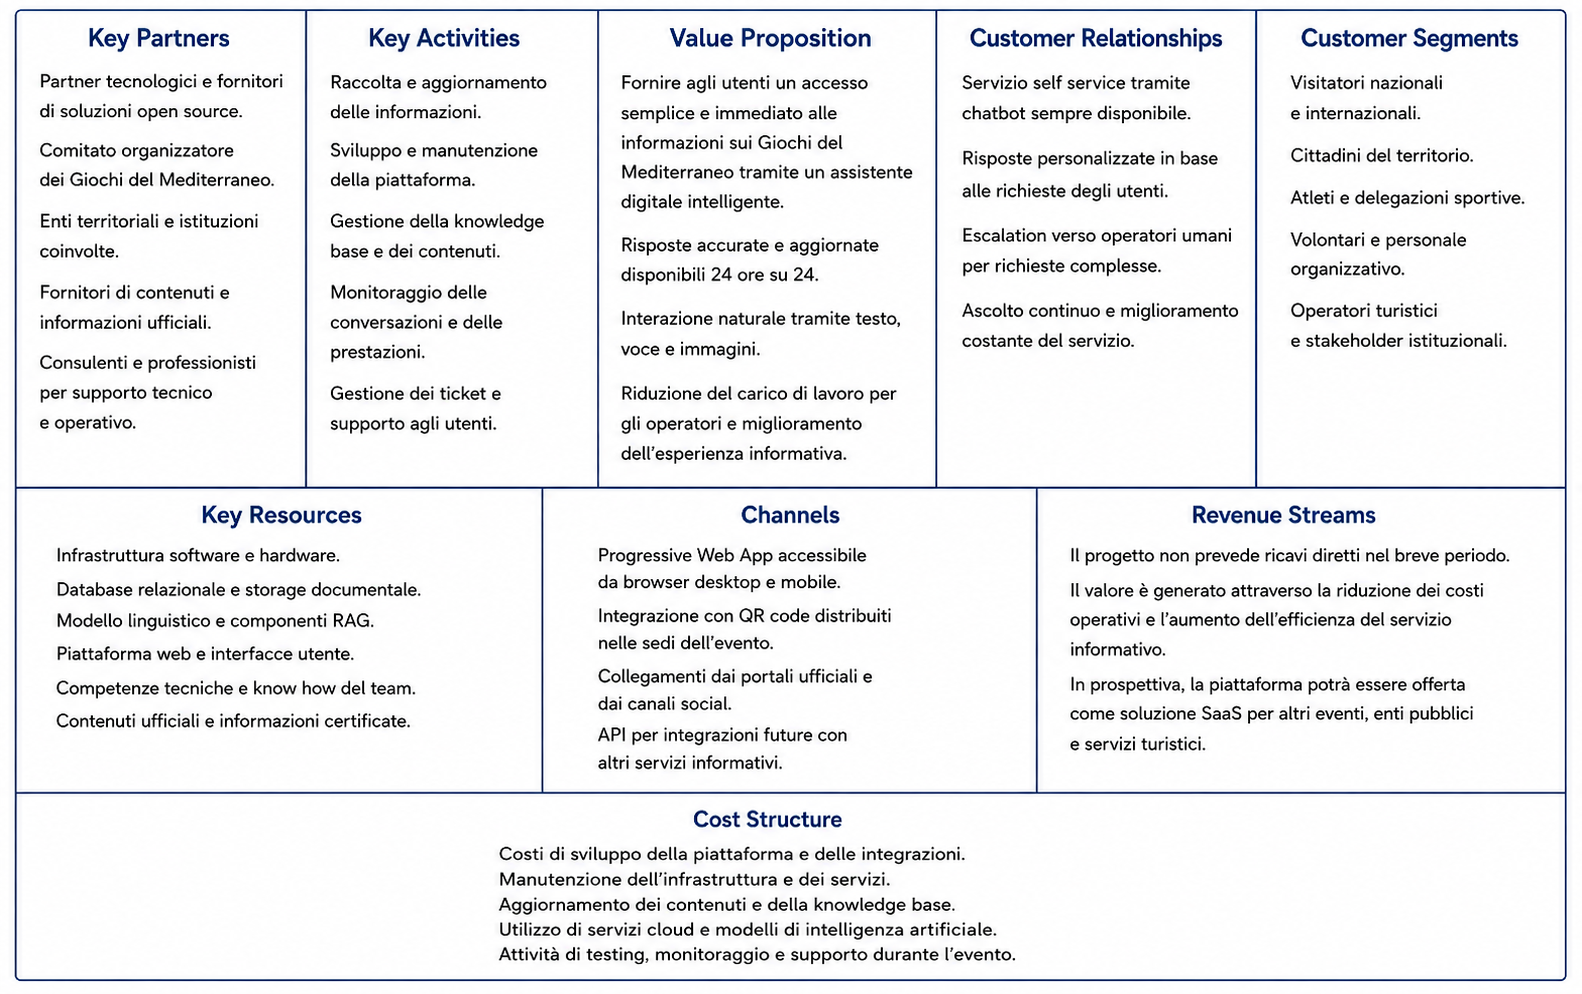
\includegraphics[width=0.98\textwidth]{images/bmc.png}
\caption{Business Model Canvas del progetto.}\label{fig:bmc}
\end{figure}

Nel canvas, la \textit{value proposition} consiste nel fornire agli utenti un accesso semplice e immediato alle informazioni attraverso un assistente intelligente e nella riduzione del carico operativo per gli operatori. Inoltre, la \textit{customer relationship} con gli utenti si basa su un modello di \textit{self-service} assistito, in cui il chatbot è sempre disponibile per le richieste comuni, mentre l’escalation verso l’operatore umano viene prevista per i casi complessi.

Dal punto di vista economico, il progetto non prevede ricavi diretti nel breve periodo, poiché nasce come soluzione di supporto informativo e operativo. Il valore viene generato soprattutto attraverso la riduzione dei costi di assistenza, l’aumento dell’efficienza del servizio e il miglioramento della qualità percepita dagli utenti.

A completamento dell’analisi di business è stata svolta anche un'analisi \textit{Strengths, Weaknesses, Opportunities and Threats} (SWOT), riportata in Figura~\ref{fig:swot}.

\begin{figure}[H]
\centering
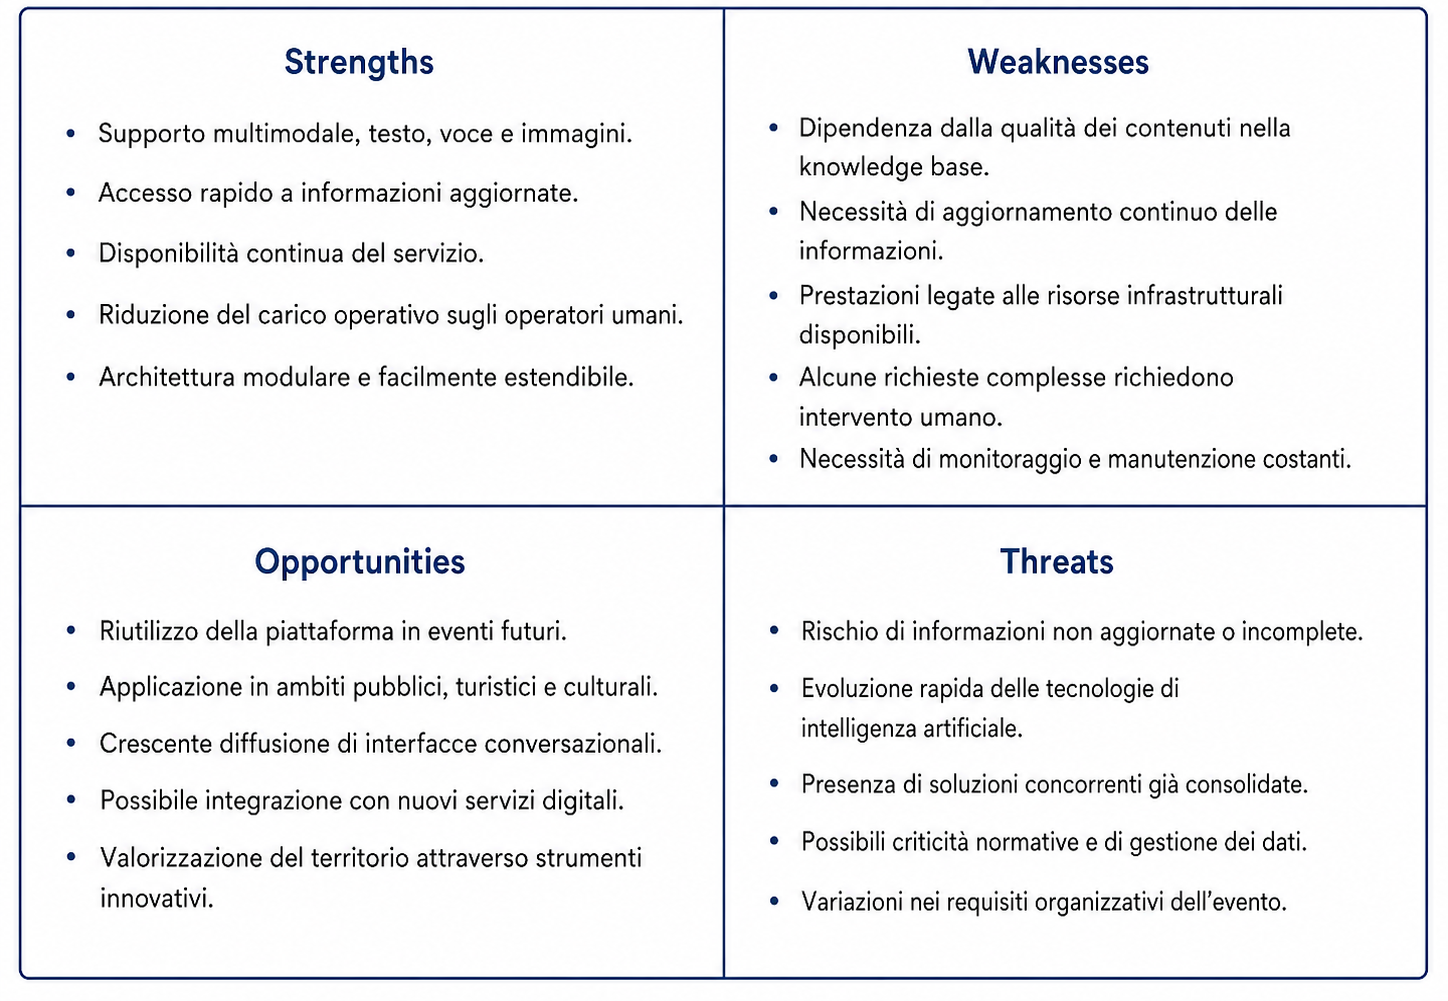
\includegraphics[width=0.98\textwidth]{images/swot.png}
\caption{Analisi SWOT del progetto.}\label{fig:swot}
\end{figure}

Tra i principali punti di forza rientrano il supporto multimodale, la disponibilità continua del servizio e la riduzione del carico operativo sugli operatori.

Le debolezze riguardano soprattutto la dipendenza dalla qualità della \textit{knowledge base} e la necessità di intervento umano in alcuni casi specifici non risolvibili in modo affidabile dal bot.

Le opportunità sono legate alla possibilità di riutilizzare la piattaforma in eventi futuri con le stesse criticità e all’evoluzione dei servizi digitali, sempre più orientati a interazioni naturali e personalizzate.

Le minacce riguardano il rischio di informazioni non aggiornate o incomplete e possibili limitazioni normative.

\section{Stato dell'arte}

Il customer care riguarda l’insieme dei processi attraverso cui un’organizzazione intercetta, comprende e risolve i bisogni degli utenti. In un modello tradizionale, l’utente cerca un’informazione e, se non riesce a trovarla, contatta un operatore umano, al quale deve spesso spiegare nuovamente il problema. Questo approccio può risultare efficace nei casi complessi, ma diventa poco efficiente quando le richieste sono numerose e ripetitive. In un modello digitale intelligente, invece, le richieste ricorrenti vengono rese accessibili in autonomia, mentre l'intervento dell'operatore è riservato ai soli casi che richiedono autonomia decisionale o competenze specialistiche.

Una prima forma di automazione del customer care è rappresentata dai chatbot tradizionali basati su regole. Questi sistemi sono efficaci quando il dominio applicativo è limitato e il flusso conversazionale può essere descritto tramite scelte predefinite, FAQ o alberi decisionali. In molti contesti aziendali possono quindi supportare attività semplici, ma risultano meno adatti in scenari complessi e dinamici.

I modelli linguistici generativi hanno ampliato le possibilità di interazione, poiché sono in grado di comprendere meglio il linguaggio naturale e produrre risposte discorsive. Tuttavia, un modello linguistico generico non possiede necessariamente informazioni aggiornate rispetto alle fonti necessarie e, in assenza di un contesto informativo adeguato, può generare contenuti non verificati. Questo fenomeno, definito allucinazione, comporta un rischio non trascurabile nel customer care: un'informazione errata è spesso più dannosa di una mancata risposta.

Per questo motivo, l’architettura RAG rappresenta una soluzione adatta per domini informativi specifici. La domanda dell’utente viene prima utilizzata per recuperare dalla base di conoscenza i documenti semanticamente più pertinenti e solo successivamente il modello linguistico genera la risposta, utilizzando le fonti recuperate come contesto.

Di seguito, in Tabella \ref{tab:valore-processo-assistenza}, sono riassunte le principali differenze tra customer care tradizionale e soluzioni digitali innovative.

\begin{longtable}{p{0.30\textwidth}p{0.30\textwidth}p{0.30\textwidth}}
\caption{Confronto tra assistenza tradizionale e progetto proposto.}\label{tab:valore-processo-assistenza}\\
\toprule
\textbf{Aspetto} & \textbf{Tradizionale} & \textbf{Automatizzato}\\
\midrule
\textbf{Accesso alle informazioni} & Ricerca manuale tra più fonti. & Punto informativo unico.\\
\textbf{Richieste ripetitive} & Gestite da operatore umano. & Gestite in autonomia quando coperte dalla KB.\\
\textbf{Casi complessi} & Non sempre arrivano strutturati. & Arrivano come ticket con contesto.\\
\textbf{Aggiornamento dei contenuti} & Dipende da modifiche manuali. & Possibile tramite interfaccia guidata e intuitiva.\\
\textbf{Impatto} & Limitata a valutazione di statistiche generiche. & Valutato tramite KPI su qualità informativa, tecnica e operativa.\\
\bottomrule
\end{longtable}